\documentclass[a4paper]{article}

%% Language and font encodings
\usepackage[french]{babel}
\usepackage[utf8]{inputenc}
\usepackage[T1]{fontenc}

\usepackage{float}

\setlength{\parindent}{1em}
%\setlength{\parskip}{1ex plus 0.5ex minus 0.2ex}
\newcommand{\hsp}{\hspace{20pt}}
\newcommand{\HRule}{\rule{\linewidth}{0.5mm}}

\usepackage{algorithm}
\usepackage[noend]{algpseudocode}
\algnewcommand{\algorithmicand}{\textbf{ and }}
\algnewcommand{\algorithmicor}{\textbf{ or }}
\algnewcommand{\OR}{\algorithmicor}
\algnewcommand{\AND}{\algorithmicand}
\algnewcommand\algorithmicforeach{\textbf{for each}}
\algdef{S}[FOR]{ForEach}[1]{\algorithmicforeach\ #1\ \algorithmicdo}
\newcommand{\myfrac}[2]{\frac{\displaystyle {#1}}{\displaystyle {#2}}}

%% Sets page size and margins
\usepackage[a4paper,top=3cm,bottom=2cm,left=3cm,right=3cm,marginparwidth=1.75cm]{geometry}

%% Useful packages
\usepackage{amsmath}
\usepackage{amssymb}
\usepackage{graphicx}
\usepackage{subcaption}
\usepackage[colorinlistoftodos]{todonotes}
\usepackage[colorlinks=true, allcolors=blue]{hyperref}
\usepackage{graphicx}

\usepackage{enumitem}
\setitemize{label=\textbullet, font=\small}

%% equations
\usepackage{amsthm}
\usepackage[retainorgcmds]{IEEEtrantools}

%% Matlab
\usepackage[framed,numbered,autolinebreaks,useliterate]{mcode}

%% theorem and proposition
\newtheorem{prop}{Proposition}
\newtheorem*{prop*}{Proposition}
\newtheorem{thm}{Théorème}

\newenvironment{myproof}[1][\proofname]{\proof[#1]\mbox{}\\*}{\endproof}

%% references shortcuts (Arthur) 
\usepackage{suffix}
\renewcommand{\eqref}[1]{équation~\ref{#1}}
\newcommand{\algoref}[1]{algorithme~\ref{#1}}
\newcommand{\figref}[1]{figure~\ref{#1}}
\newcommand{\tabref}[1]{tableau~\ref{#1}}
\newcommand{\secref}[1]{section~\ref{#1}}
\newcommand{\probref}[1]{problème~\ref{#1}}
\newcommand{\propref}[1]{proposition~\ref{#1}}
\newcommand{\theoremref}[1]{théorème~\ref{#1}}
\newcommand{\chapref}[1]{chapitre~\ref{#1}}
\WithSuffix\newcommand\algoref*[1]{algorithme~\ref{#1} p.~\pageref{#1}}
\WithSuffix\newcommand\figref*[1]{figure~\ref{#1} p.~\pageref{#1}}
\WithSuffix\newcommand\eqref*[1]{équation~\ref{#1} p.~\pageref{#1}}
\WithSuffix\newcommand\tabref*[1]{tableau~\ref{#1} p.~\pageref{#1}}
\WithSuffix\newcommand\secref*[1]{section~\ref{#1} p.~\pageref{#1}}
\WithSuffix\newcommand\probref*[1]{problème~\ref{#1} p.~\pageref{#1}}
\WithSuffix\newcommand\propref*[1]{proposition~\ref{#1} p.~\pageref{#1}}
\WithSuffix\newcommand\chapref*[1]{chapitre~\ref{#1} p.~\pageref{#1}}

\usepackage[backend=biber,uniquename=init,giveninits=true,
             %% "et al" pour > deux auteurs, & pour exactement 2
             uniquelist=false,maxcitenames=2,mincitenames=1,maxbibnames=99,
             isbn=false,url=false,doi=false,bibstyle=numeric
]{biblatex}
\addbibresource{references.bib}

\begin{document}

\begin{titlepage}
  \begin{center}

      \makebox[0.5\textwidth][r]{%
        
\includegraphics[width=0.33\textwidth]{images/sorbonne.png}%
    }%

      \vspace{4cm}
    % Title
    \HRule \\[0.4cm]
    { \huge \bfseries BIMA\\[0.4cm] }

      \textsc{\LARGE Mini rapport TP7}\\[0.4cm]

    \HRule \\[0.8cm]

    % Author and supervisor
    \begin{minipage}{0.4\textwidth}
      \begin{flushleft} \large
        Kim-Anh Laura \textsc{Nguyen}\\
        \large
        Arij \textsc{Riabi}\\
        M1 DAC\\
        Promo 2018-2019 \\
      \end{flushleft}
    \end{minipage}
    \begin{minipage}{0.5\textwidth}
      \begin{flushright} \large
        \emph{Enseignant :} Dominique \textsc{Béréziat}\\
      \end{flushright}
    \end{minipage}

      \vspace{2cm}

  \end{center}
  %\end{sffamily}
\end{titlepage}
%\maketitle

\newpage

\section*{Exercice 1 - Expérimentation du découpage}

\begin{figure}[H]
    \centering
     
    \begin{subfigure}[c]{0.6\textwidth}
        \centering
        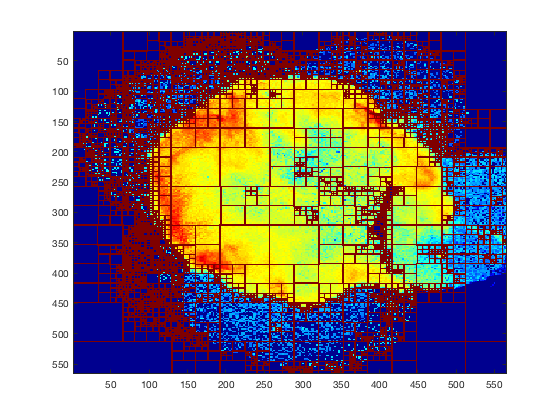
\includegraphics[width=\textwidth]{images/ex1_cygnus.png}
        \caption{\texttt{cygnus.tif}}
    \label{subfig:ex1_cygnus}
    \end{subfigure}
    \begin{subfigure}[c]{0.6\textwidth}
        \centering
        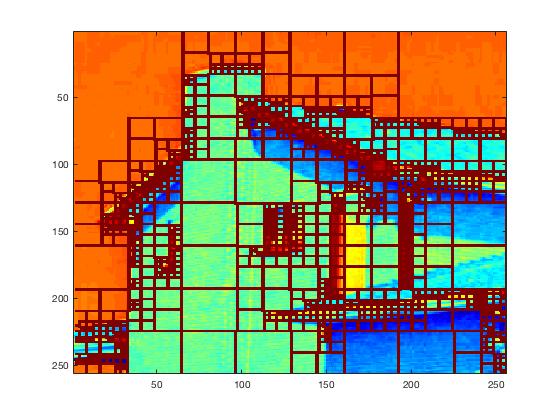
\includegraphics[width=\textwidth]{images/ex1_house.png}
        \caption{\texttt{house.png}}
        \label{subfig:ex1_house}
    \end{subfigure}
    \begin{subfigure}[c]{0.6\textwidth}
        \centering
        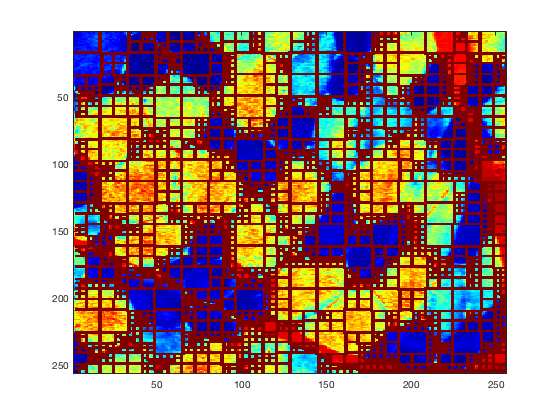
\includegraphics[width=\textwidth]{images/ex1_muscle.png}
        \caption{\texttt{muscle.pgm}}
    \label{subfig:ex1_muscle}
    \end{subfigure}

    \caption{Segmentation de plusieurs images selon un découpage
    \texttt{Quadtree}} 
    \label{fig:ex1}
\end{figure}

\section*{Exercice 2 - Expérimentation de la fusion}

\begin{figure}[H]
    \centering
     
    \begin{subfigure}[c]{0.6\textwidth}
        \centering
        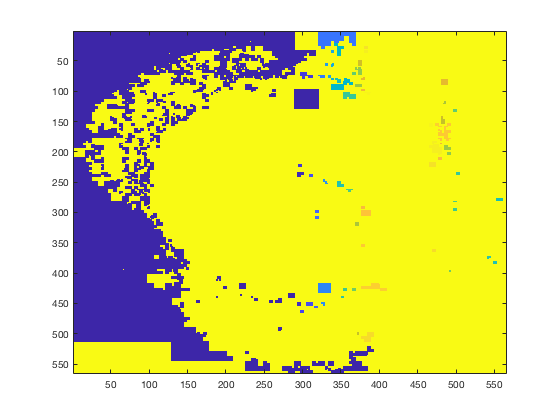
\includegraphics[width=\textwidth]{images/ex2_cygnus.png}
        \caption{\texttt{cygnus.tif}}
    \label{subfig:ex2_cygnus}
    \end{subfigure}
    \begin{subfigure}[c]{0.6\textwidth}
        \centering
        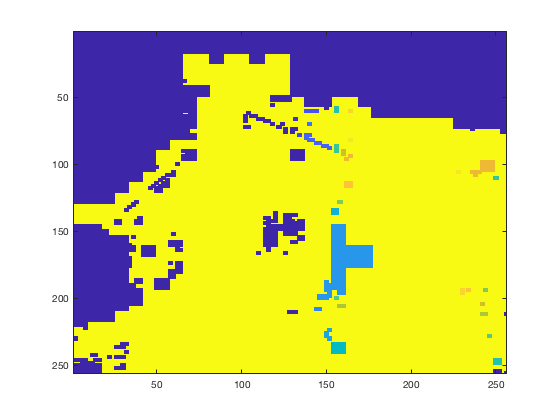
\includegraphics[width=\textwidth]{images/ex2_house.png}
        \caption{\texttt{house.png}}
        \label{subfig:ex2_cygnus}
    \end{subfigure}
    \begin{subfigure}[c]{0.6\textwidth}
        \centering
        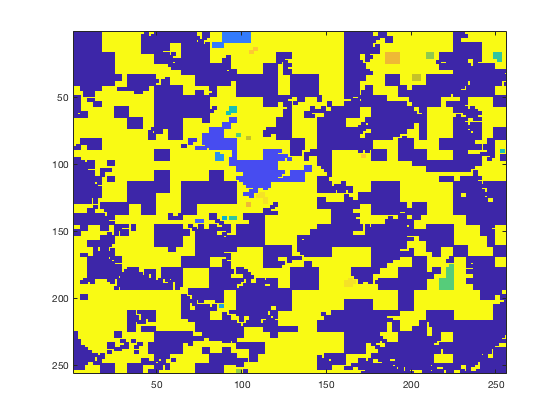
\includegraphics[width=\textwidth]{images/ex2_muscle.png}
        \caption{\texttt{muscle.pgm}}
    \label{subfig:ex2muscle}
    \end{subfigure}

    \caption{Application de l'algorithme \texttt{split merge} (avec fusion locale) de plusieurs
    images selon un découpage \texttt{Quadtree}}
    \label{fig:ex2}

    %\begin{subfigure}[c]{0.3\textwidth}
    %    \centering
    %    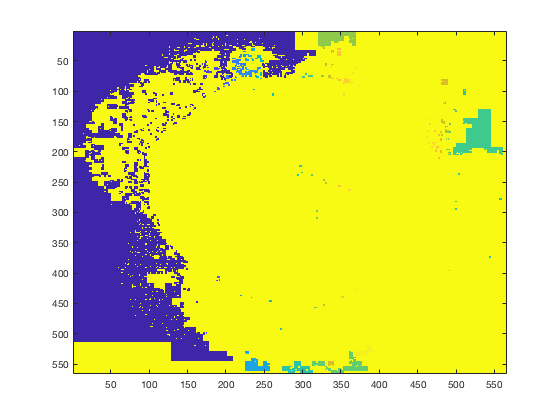
\includegraphics[width=\textwidth]{images/ex2q3_cygnus.png}
    %    \caption{\texttt{cygnus.tif} (fusion globale)}
    %\label{subfig:ex2q3_cygnus}
    %\end{subfigure}
    %\begin{subfigure}[c]{0.3\textwidth}
    %    \centering
    %    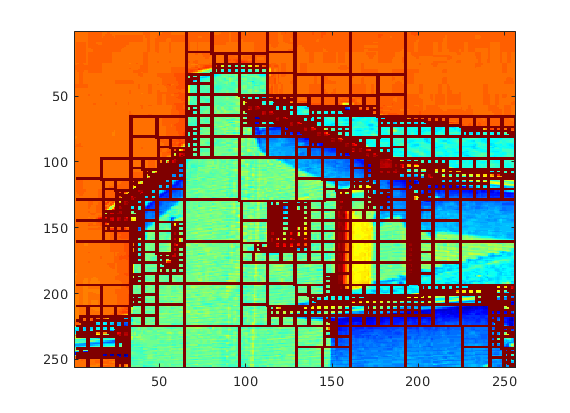
\includegraphics[width=\textwidth]{images/ex2q3_house.png}
    %    \caption{\texttt{house.png} (fusion globale)}
    %    \label{subfig:ex2q3_cygnus}
    %\end{subfigure}
    %\begin{subfigure}[c]{0.3\textwidth}
    %    \centering
    %    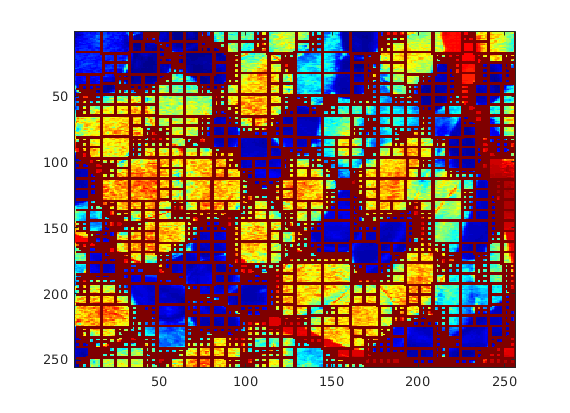
\includegraphics[width=\textwidth]{images/ex2q3_muscle.png}
    %    \caption{\texttt{muscle.pgm} (fusion globale)}
    %\label{subfig:ex2q4muscle}
    %\end{subfigure}

    %\caption{Application de l'algorithme \texttt{split merge} de plusieurs
    %images selon un découpage \texttt{Quadtree}} 
    %\label{fig:ex1}
\end{figure}

\begin{figure}[H]
    \centering
     
    \begin{subfigure}[c]{0.6\textwidth}
        \centering
        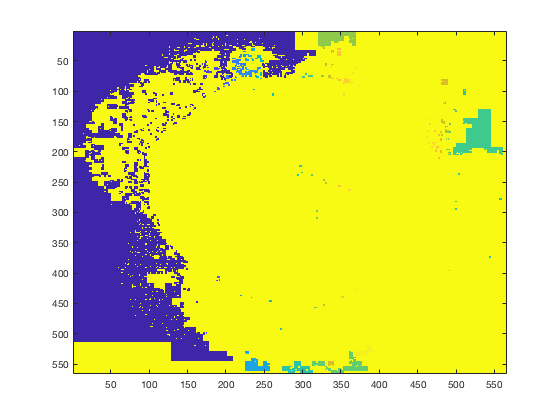
\includegraphics[width=\textwidth]{images/ex2q3_cygnus.png}
        \caption{\texttt{cygnus.tif}}
    \label{subfig:ex2q3_cygnus}
    \end{subfigure}

    %\begin{subfigure}[c]{0.6\textwidth}
    %    \centering
    %    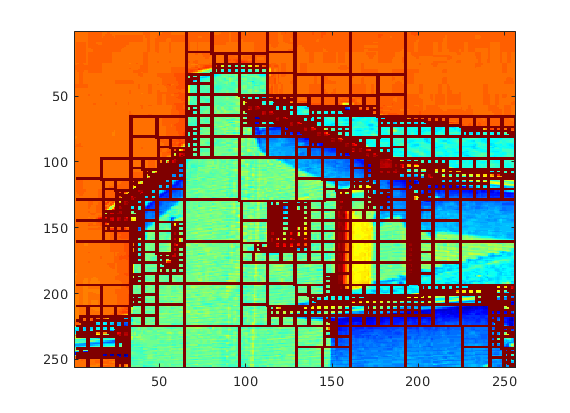
\includegraphics[width=\textwidth]{images/ex2q3_house.png}
    %    \caption{\texttt{house.png}}
    %    \label{subfig:ex2q3_house}
    %\end{subfigure}
    %\begin{subfigure}[c]{0.6\textwidth}
    %    \centering
    %    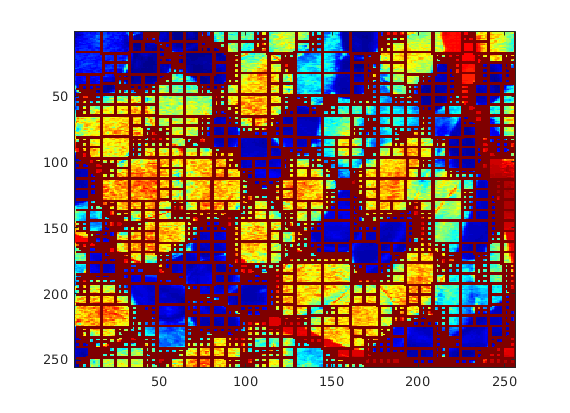
\includegraphics[width=\textwidth]{images/ex2q3_muscle.png}
    %    \caption{\texttt{muscle.pgm}}
    %\label{subfig:ex2q3_muscle}
    %\end{subfigure}
    
    \caption{Application de l'algorithme \texttt{split merge} (avec fusion
    globale) de \texttt{cygnus.tif} selon un découpage \texttt{Quadtree}}
    \label{fig:ex2q3}
\end{figure}

\end{document}
